\section*{Exploitation des données}

\addcontentsline{toc}{chapter}{Exploitation des données}

\subsection*{Stratégie de clusterisation}
\addcontentsline{toc}{section}{Stratégie de clusterisation}
Nous avons choisi de réaliser un clustering hiérarchique car l'attribution de scores aux protéines nous paraissait particulièrement complexe dans le cas de données non numériques. 

\begin{figure}
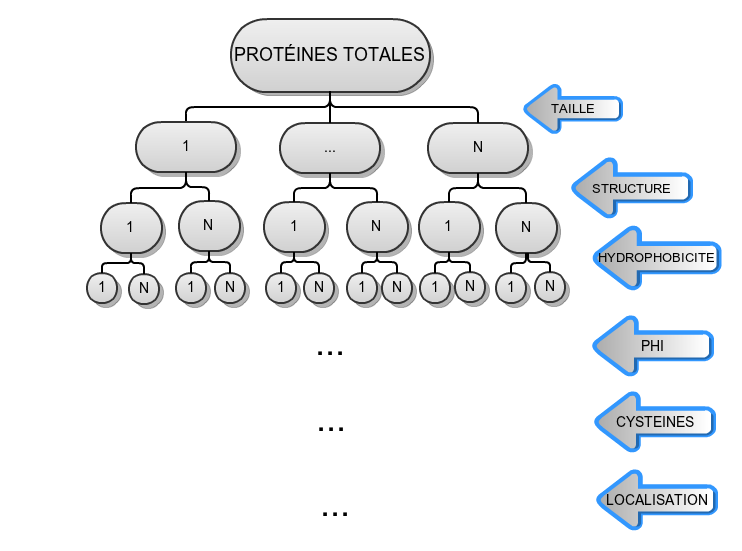
\includegraphics[scale=0.5]{Datamining.png}
\caption{Schéma des niveaux de clusterisation} 
\end{figure}

\subsubsection*{Clusters de taille}
Pour que la formation des clusters de taille se fasse rapidement, nous avons tout d'abord décidé de trier les protéines par longueur croissante. \\
Puis nous les avons regroupées dans des cluster de 250 éléments. Nous avons choisi ce nombre car le temps de traitement pour le calcul des clusters suivants était trop long (évolution exponentielle du temps de traitement).

\subsubsection*{Autres clusters}
Dans un premier temps, nous avons calculé la distance entre deux protéines gr\^ace à la distance de Manhattan.\\
Par exemple, pour les tissus, nous comparons la similarité entre deux listes (le nombre de tissus communs entre les deux protéines divisé par le nombre de tissus maximum entre les deux protéines).\\
Pour les structures secondaires, le calcul des distances s'effectue entre trois paramètres (helix, strand, turn) suivant la formule: 
    $d(A,B)=|X_B-X_A|+|Y_B-Y_A|+|Z_B-Z_A|$.\\

Puis, à partir de ces distances, nous avons établi une matrice (matrice de dissimilarité) que nous réduisons petit à petit en regroupant les protéines qui ont les distances les plus proches. Nous avons répété l'opération jusqu'à diviser chaque cluster en quatre nouveaux clusters (algorithme AGNES). Cette méthode permet de ne pas avoir à fixer de taille aux clusters obtenus, cependant il faut décider arbitrairement du niveau d'arr\^et de la clusterisation.

\begin{figure}
\begin{center}
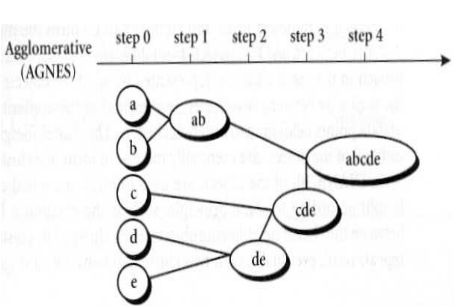
\includegraphics[scale=0.6]{agnes.png}
\caption{Méthode de clusterisation AGNES}
\end{center}
\end{figure}



